% this chapter is basically covered by
% - Optimizations https://cds.cern.ch/record/2912217
% - Acts integration https://cds.cern.ch/record/2921878
% - Expected tracking performance https://arxiv.org/abs/2412.15090
% - TDR https://cds.cern.ch/record/2802799

The new inner tracking detector (ITk) for the ATLAS Phase-2 upgrade is designed to cope with the high instantaneous luminosity and pileup conditions expected in the High-Luminosity Large Hadron Collider (HL-LHC) era. The ITk is a full-silicon detector and will be composed of a pixel \cite{itk-pixel-tdr} and a strip \cite{itk-strip-tdr} subsystem. This upgrade is not only challening for the detector design, construction, and opteration, but also the track reconstruction software. The ATLAS collaboration is corrently working on upgrading the reconstruction software for Run 4, which is the first run with the new detector. This includes the migration of the track reconstruction to use the Acts toolkit, for both the inner detector and the muon spectrometer. Part of the work on this thesis was to integrate the Acts track finding algorithm into the ATLAS track reconstruction software, which was a joint effort and performed in close collaboration with the Acts-ITk team.

In addition to the ongoing software upgrade, the ATLAS collaboration is developing a new trigger system for Run 4 and is currently evaluating various hardware technologies for implementing the High-Level Trigger (HLT). One of the proposed solutions is a CPU-based track reconstruction chain based on the Acts toolkit. Alternative approaches under consideration include GPU- and FPGA-based implementations.

\section{Acts-based track reconstruction chain}

The Acts-based track reconstruction chain is planned to use the same reconstruction steps as the already existing reconstruction chain, referred to as the \textit{legacy chain} here. The legacy chain is based on Run 3 reconstruction \cite{atlas-sac-run3} and tuned to some degree for Run 4. The main motivation for the Acts-based chain is to increase maintainability and potentially performance. The ATLAS track reconsturction software was written in the early 2000s and its authors are practically no longer available. New people entering the collaboration are faced with a large amount of legacy code which is poorly documented and difficult to understand. For this reason, the ATLAS collaboration decided to adopt the Acts toolkit for the Run 4 track reconstruction, as it promises to be modern, maintainable, documented, and efficient from the start.

To achieve this, some reconstruction algorithms have been ported from legacy code to Acts and validated against the existing legacy chain. An example for this is the triplet seeding algorithm. Other algorithms, like the Kalman-based track finding and fitting, have been implemented from scratch in Acts, using literature and experience from the legacy chain. One of the main benefits of Acts is its experiment-agnostic design, which allows to use the same code across different experiments. Other experiments can benefit from existing, validated reconstruction code, and potentially contribute to the development of the Acts toolkit. In this case, ATLAS will benefit from the experience of other experiments.

The legacy and Acts-based reconstruction chain are very close to what was described in the introduction in Section \ref{sec:intro/reco/reco-steps}. The main pass, which reconstructs tracks from the primary interactions, starts from raw sensor data. The raw data is clustered and measurements are formed. The measurements are used to form spacepoints, which are the input to the seeding algorithm. The seeding algorithm finds potential starting points for tracks, which are used by the track finding algorithm to find track candidates. The clusterization, spacepoint formation, and seeding steps are performed separately for pixels and stips. The track finding step combines pixel and stip seeds to form a single track collection.

One main difference between the legacy and Acts-based chain is the track finding algorithm. While the legacy chain focuses only on finding compatible measurements, the Acts-based chain deploys a fully-fledged Kalman filter to not only find but also fit tracks simultaneously. Due to this, the Acts-based chain does not need a separate fitting step, which is required in the legacy chain.

Apart from that, the Acts-based chain only deploys a simplistic ambiguity resolution algorithm for now, which is based on the greedy approach described in Section \ref{sec:dev/general/greedy-ambiguity-resolution}. The legacy chain uses a more sophisticated ambiguity resolution algorithm, which is also able to resolve cluster ambiguities and refit tracks based on this information. How this will be implemented in the Acts-based chain is currently under investigation.

The Acts-based track reconstruction chain can be used for offline reconstruction, as well as for the HLT. The HLT is part of the ATLAS trigger system and makes the final decision on whether an event is saved to disk or discarded forever. The tracking chain used for offline is called \textit{default chain}, while the one used for the HLT is called \textit{fast chain} \cite{pubnote-2019-041}. The main differences between the two chains are the reconstruction cuts and that the fast chain only considers pixel seeds.

\section{CPU performance optimizations}
\label{sec:perf/itk/cpu-performance}

Since compute resources will be limited for reconstructing the large amount of data expected from the HL-LHC, the Acts-based chain does not only need to deliver similar physics performance as the legacy chain, but perform at least as well as the legacy chain in terms of CPU time \cite{atlas-hl-lhc-computing-cdr}\cite{atlas-tdr-029-add}. To achieve this, the Acts-based chain has been optimized over several iterations. This was carried out by the Acts-ITk team and as part of the work on this thesis. Some of these optimizations were performed directly in Acts and have already been described in Chapter \ref{ch:dev/track_finding}.

\begin{figure}[h]
    \centering
    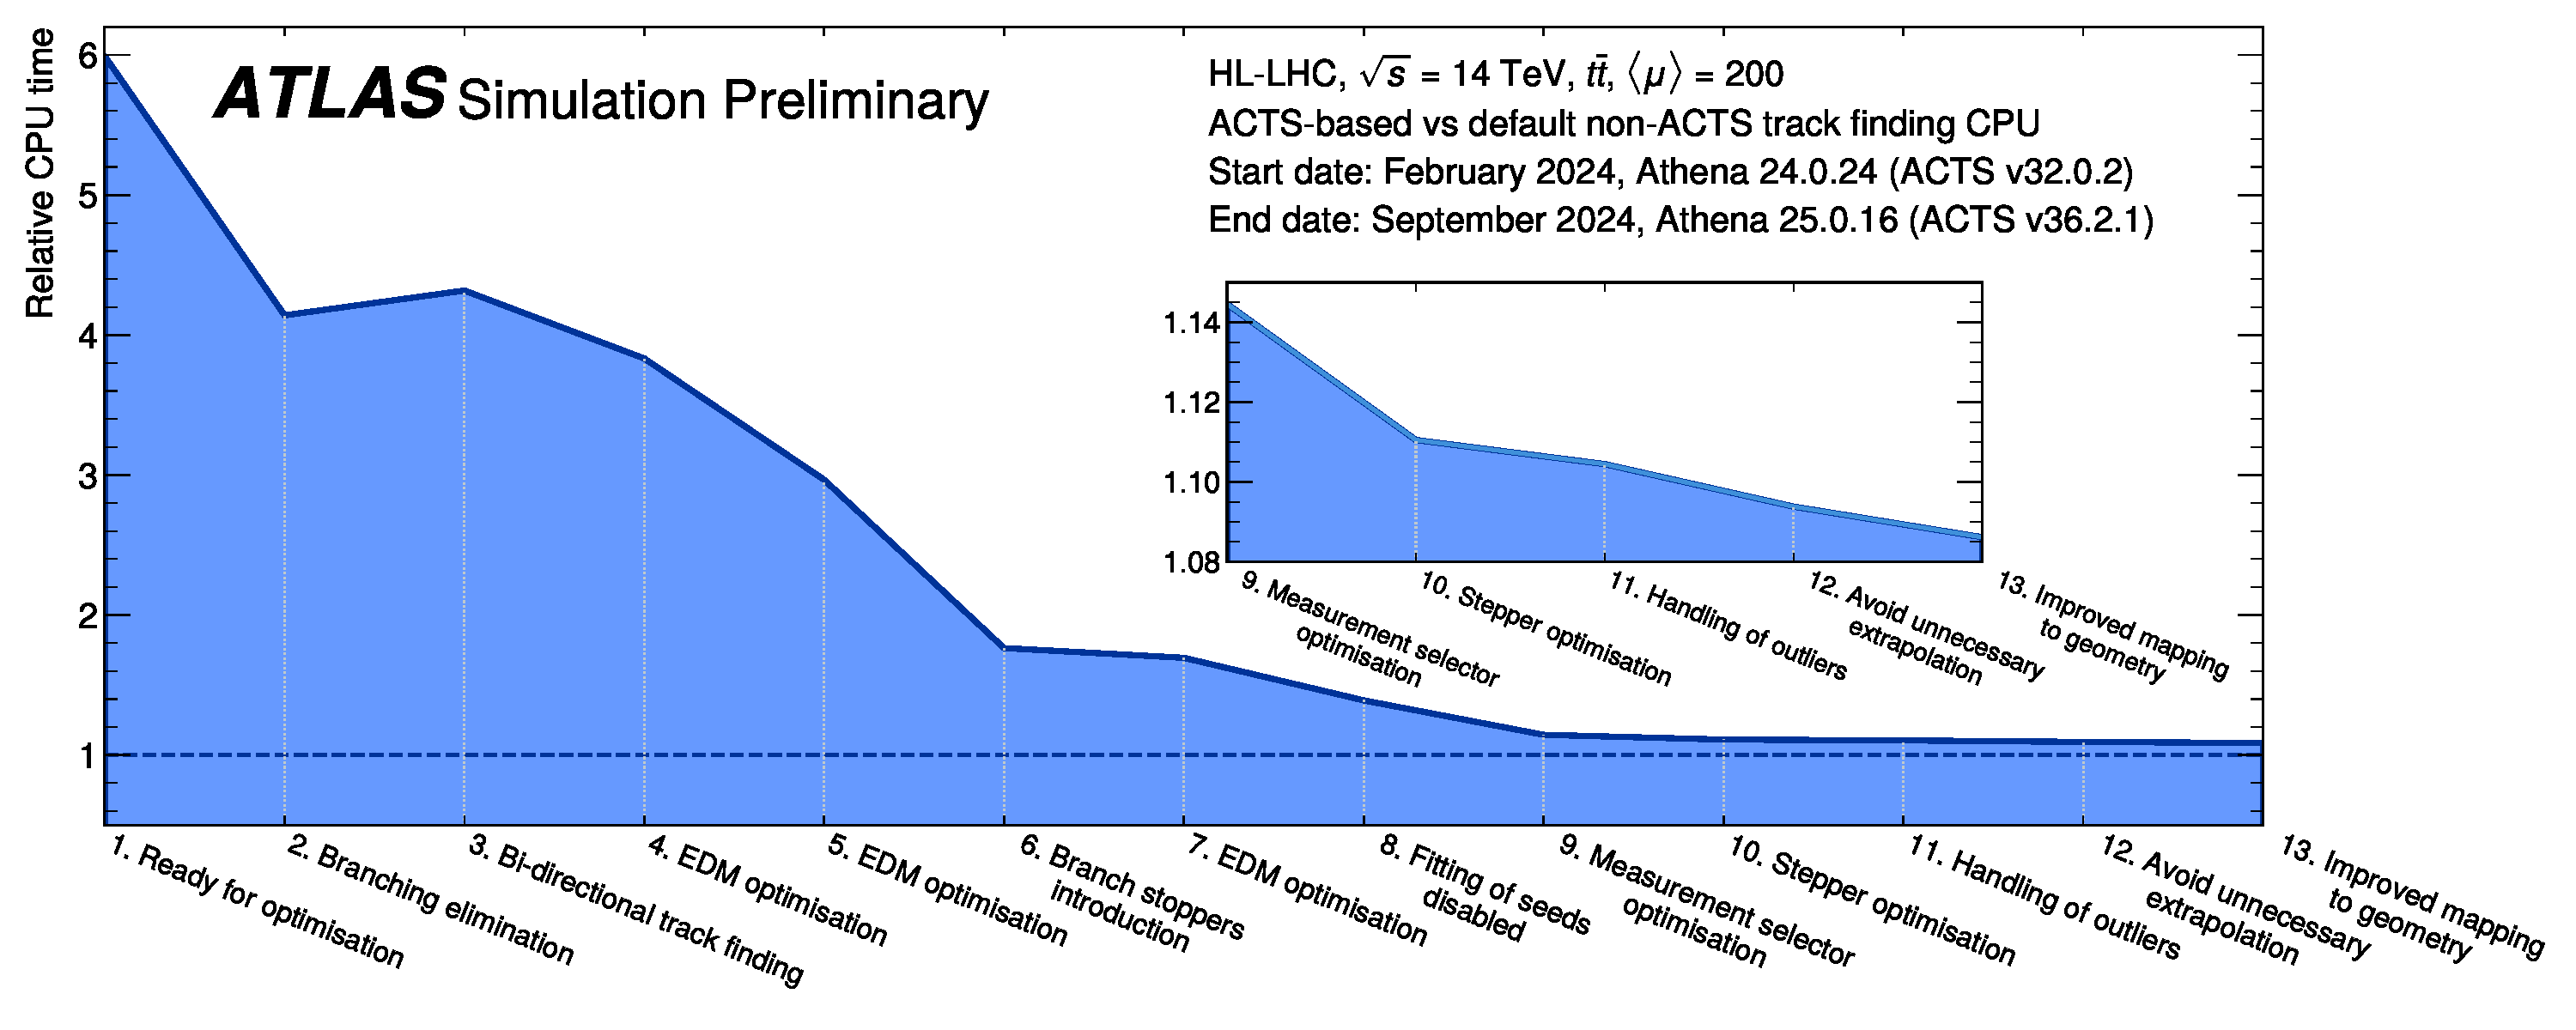
\includegraphics[width=1.15\textwidth]{parts/3_performance/12_itk-performance/figures/cpu_improvements.pdf}
    \caption{Incremental improvements to the compute time for reconstructing \ttbar events at $\langle \mu \rangle$ = 200 with the ATLAS reconstruction software Athena \cite{pubnote-2024-017}. The CPU time shown only accounts for track finding, and it is relative to the legacy counterpart. A zoomed version of the last 5 data points is also shown.}
    \label{fig:perf/itk/cpu-improvements}
\end{figure}

Figure \ref{fig:perf/itk/cpu-improvements} shows the incremental improvements to the compute time for reconstructing \ttbar events at $\langle \mu \rangle$ = 200 with the ATLAS reconstruction software Athena. This has beed documented in \textcite{pubnote-2024-017} and is partially recapitulated and expanded here. The starting date for the plot is 15 February 2024, using Athena 24.0.24 (Acts v32.0.2). The relevant improvements are listed in chronological order on the horizontal axis of the plot and described below. The last data point on the plot corresponds to the running time obtained on 10 September 2024 using Athena 25.0.16 (Acts v36.2.1). The symbol $\dagger$ indicates a major contribution to the item was made during the work on this thesis.

\begin{enumerate}
    \item \textbf{Ready for optimization}: the starting point of the optimizations, corresponding to the first  fullyfunctional version of the Acts-based ITk track reconstruction deployed in Athena 24.0.24 (Acts v32.0.2) on 15 February 2024. With this version of the code, the Acts track finding was measured to be six times slower than the legacy one.
    \item \textbf{Branching elimination $\dagger$}: the combinatorial Kalman filter is configured to only consider a single branch. Hence, proving one input seed can at most result in a single track candidate. This is justified by the fact that the triplet seeding algorithm already explors the measurement combinatorics and the track finding does not need to do this as well.
    \item \textbf{Bi-directional track finding $\dagger$}: enabling track finding to search for measurements both outward (i.e. away from the interaction point) and inward. This is described in more detail in Section \ref{sec:dev/trackfinding/two-way}.
    \item \textbf{EDM optimization}: improved storage and access of the seed containers.
    \item \textbf{EDM optimization}: better usage of internal representation of track containers.
    \item \textbf{Branch stoppers introduction $\dagger$}: usage of early branch-aborting conditions to stop the track finding and decide whether to keep the track candidate.
    \item \textbf{EDM optimization}: simplification of measurement access from track states. These developments led to a more general improvement of measurement projection in Acts described in Section \ref{sec:dev/general/measurement-projection} $\dagger$.
    \item \textbf{Fitting of seeds disabled $\dagger$}: avoiding seed parameter refinement using a Kalman filter. This was shown not to be critical for the track finding performance, especially in the pixels.
    \item \textbf{Measurement selector optimization}: improved selection and calibration of measurements during track state creation for the combinatorial Kalman filter.
    \item \textbf{Stepper optimizations $\dagger$}: faster implementation of the numerical integration and the Jacobian and covariance transport. This is described in more detail in Section \ref{sec:dev/stepper/sympy}.
    \item \textbf{Handling of outliers $\dagger$}: implementation of a dedicated outlier compatibility criterion. Define a maximum number of outliers allowed per track and stop track finding earlier if the limit is exceeded.
    \item \textbf{Avoid unnecessary extrapolation $\dagger$}: avoiding unnecessary extrapolation at the end of track finding, in case this is already performed by the inward extension.
    \item \textbf{Improved mapping to geometry}: improved mapping of detector elements and measurements to tracking geometry surfaces.
\end{enumerate}

At the end of the optimizations, the Acts-based track finding was measured to be about 8\% slower than the legacy counterpart. This is a significant improvement compared to the starting point. Given the fact that the Acts-based chain does not need a separate fitting step, the overall performance of the Acts-based chain is expected to be better than the legacy chain. However, not all algorithms have been ported to Acts yet, including a more sophisticated ambiguity resolution algorithm that deals with cluster ambiguities. Only after the chains are feature equivalent, a fair comparison can be made. This is an ongoing effort.

Given the current workload of the track finding algorithm, it appears that its CPU performance cannot be significantly improved further. A potential bottleneck is the triplet seeding algorithm, which produces a large number of fake seeds. These fakes are filtered out by the track finding algorithm which consumes additional CPU time. Other seeding algorithms exist, which produce less fakes and show promising CPU performance \cite{acts-gbts}. However, these algorithms are not yet available in Acts. The Acts-ITk team is currently working on integrating these algorithms into Acts and the Acts-based ITk chain.

\section{Physics performance}
\label{sec:perf/itk/physics-performance}

The physics performance of the Acts-based chain is continously evaluated aginst the legacy chain. The goal is to achieve similar or better performance in terms of track reconstruction efficiency, fakes, and resolution. The performance is evaluated using simulated events, which are reconstructed with both chains. An extensive evaluation of the expected tracking performance of the legacy chain is available in \textcite{itk-tracking-performance}. For the evaluation in the following only single muon and \ttbar samples were used. The single muon sample is used to evaluate the track finding and fitting performance in a clean environment, while the \ttbar sample is used to evaluate the finding performance in a more realistic environment with pileup.

\begin{figure}[H]
    \centering
    \begin{subfigure}[b]{1.0\textwidth}
        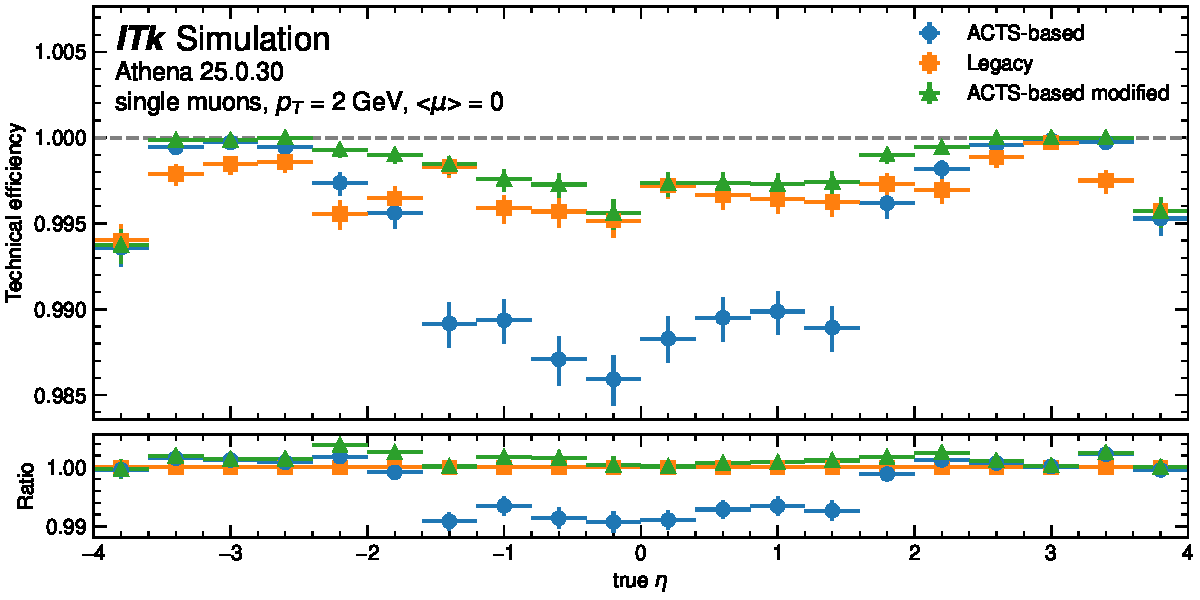
\includegraphics[width=1.0\linewidth]{parts/3_performance/12_itk-performance/figures/default_mod_single_mu_pt2_eff_vs_eta.pdf}
    \end{subfigure}
    \begin{subfigure}[b]{1.0\textwidth}
        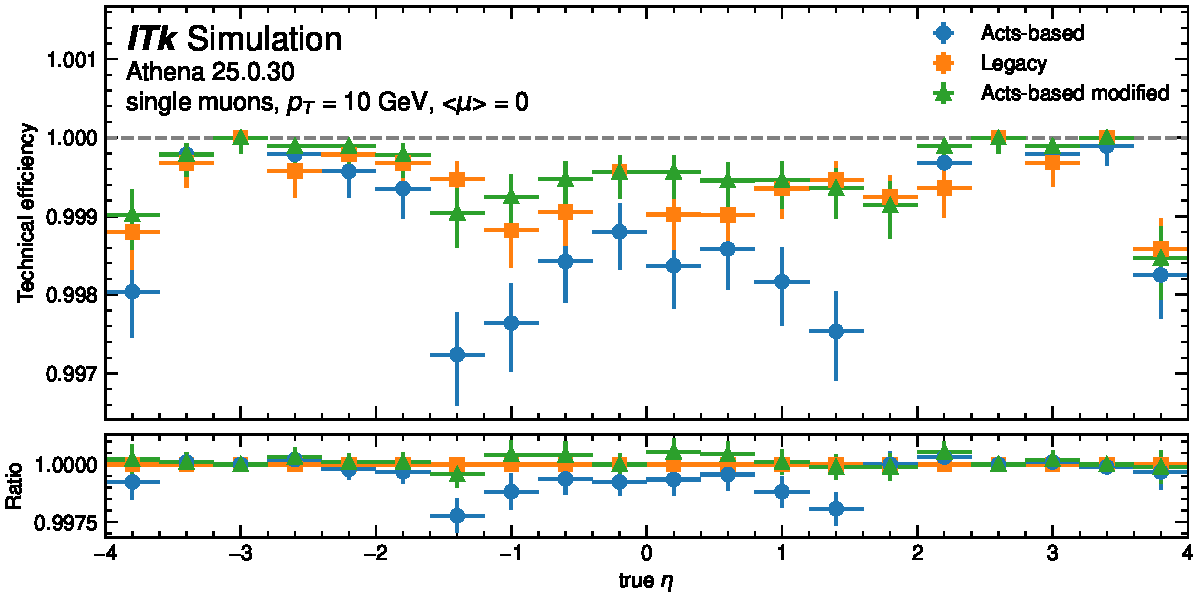
\includegraphics[width=1.0\linewidth]{parts/3_performance/12_itk-performance/figures/default_mod_single_mu_pt10_eff_vs_eta.pdf}
    \end{subfigure}
    \caption{Technical track efficiency as a function of true $\eta$ for single $\mu$ with $p_T = 2,10$ GeV for the Acts-based and legacy chain.}
    \label{fig:perf/itk/eff-single-mu}
\end{figure}

Figure \ref{fig:perf/itk/eff-single-mu} shows the technical track efficiency as a function of true $\eta$ for single muons with $p_T = 2,10$ GeV for the Acts-based and legacy chain. The Acts-based chain shows good performance for the endcap region $|\eta| > 1.5$, but significant inefficiency in the barrel region $|\eta| < 1.5$ compared to the legacy chain. A modified Acts-based chain is included in the plots which uses a relaxed $\chi^2$ threshold of 100 instead of 25 to assign measurements during track finding. This is a temporary solution to improve the performance in the barrel region. The modified Acts-based chain shows a significant improvement compared to the unmodified Acts-based chain in the barrel region and is consistently better than the legacy chain.

\begin{figure}[H]
    \centering
    \begin{subfigure}[b]{1.0\textwidth}
        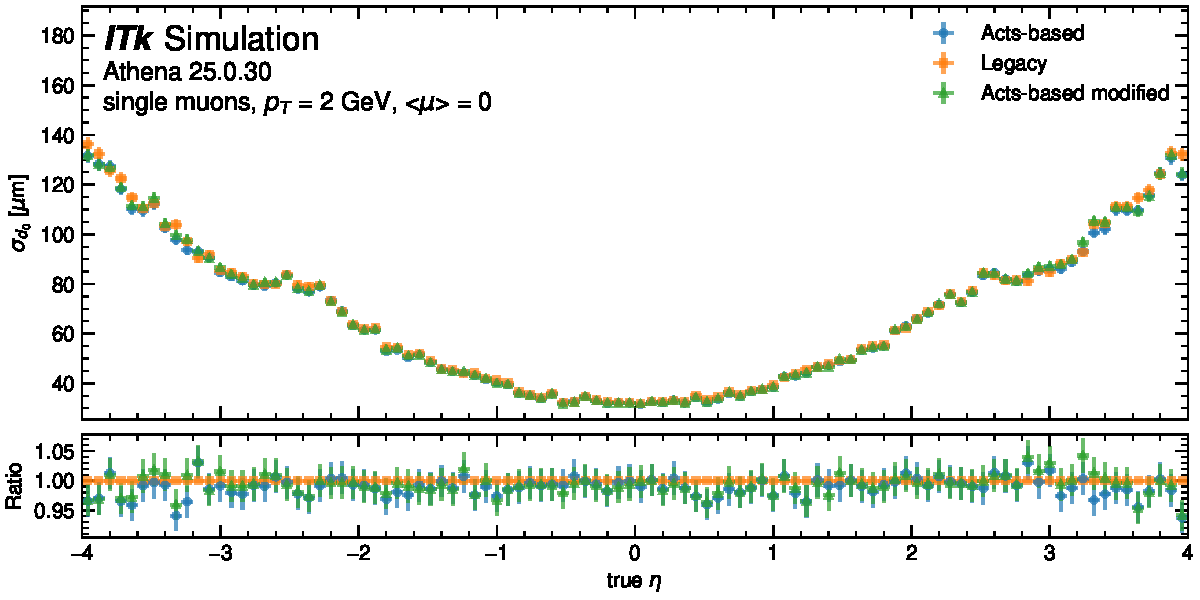
\includegraphics[width=1.0\linewidth]{parts/3_performance/12_itk-performance/figures/default_mod_single_mu_pt2_res_d0_vs_eta.pdf}
    \end{subfigure}
    \begin{subfigure}[b]{1.0\textwidth}
        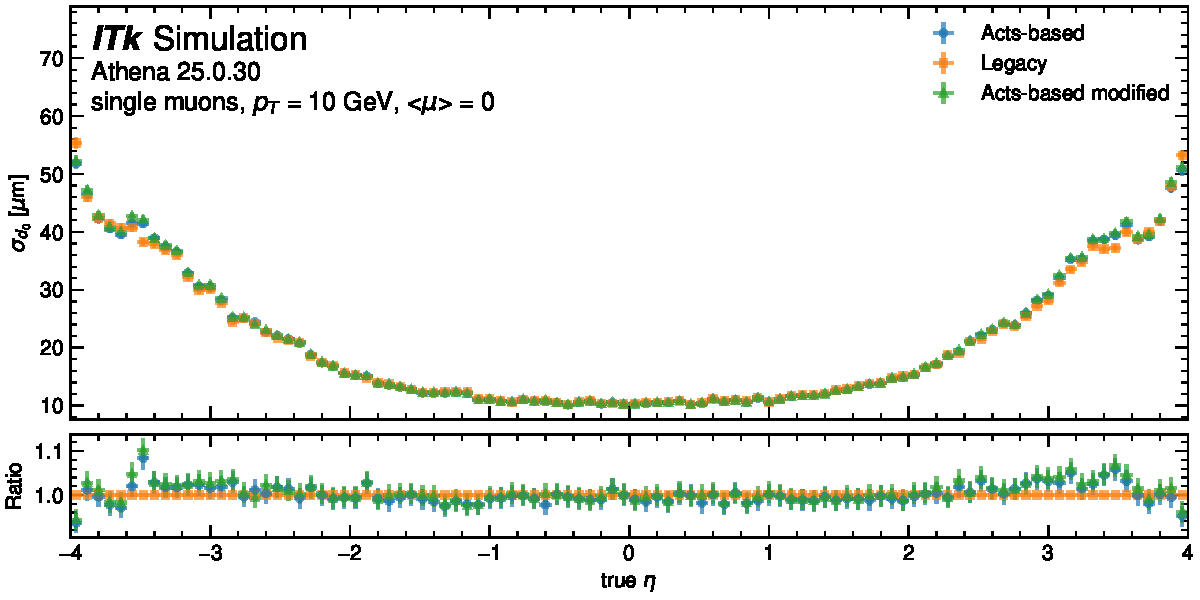
\includegraphics[width=1.0\linewidth]{parts/3_performance/12_itk-performance/figures/default_mod_single_mu_pt10_res_d0_vs_eta.pdf}
    \end{subfigure}
    \caption{Track resolution of $d_0$ as a function of true $\eta$ for single $\mu$ with $p_T = 2,10$ GeV for the Acts-based and legacy chain.}
    \label{fig:perf/itk/res-single-mu}
\end{figure}

Figure \ref{fig:perf/itk/res-single-mu} shows the resolution of the transverse impact parameter $d_0$ as a function of true $\eta$ for single $\mu$ with $p_T = 2,10$ GeV for the Acts-based and legacy chain. The resolution is similar and within 5\% for almost the full $\eta$ range. Differences in the resolution can be caused by different hit contents of the tracks after finding and different fitting algorithms and implementations.

\begin{figure}[H]
    \centering
    \begin{subfigure}[b]{1.0\textwidth}
        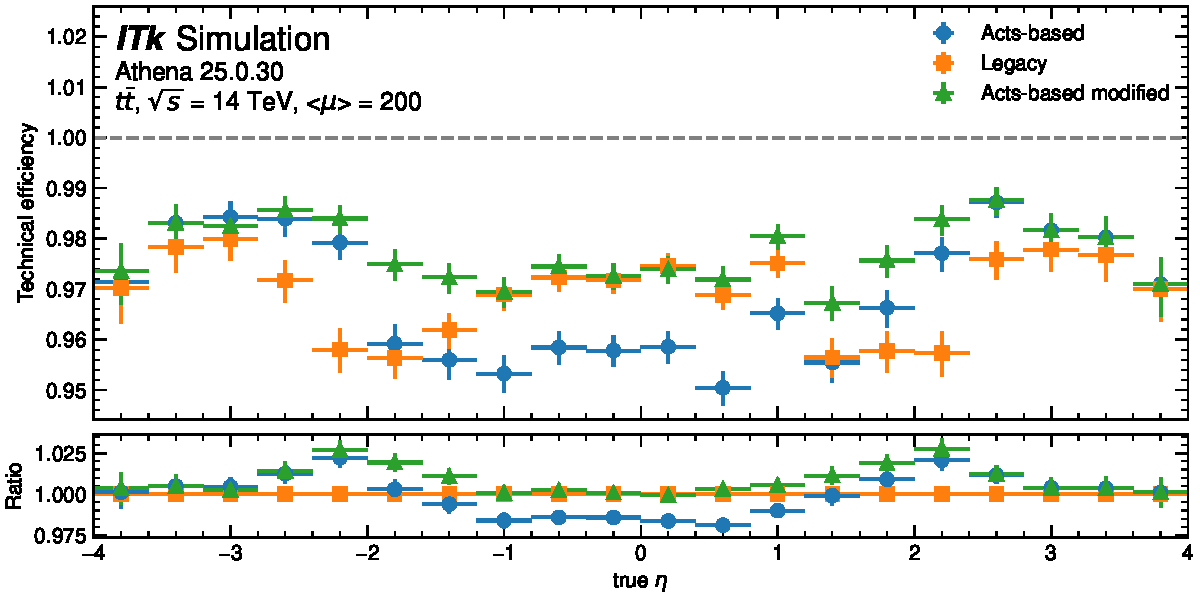
\includegraphics[width=1.0\linewidth]{parts/3_performance/12_itk-performance/figures/default_mod_ttbar_pu200_eff_vs_eta.pdf}
    \end{subfigure}
    \begin{subfigure}[b]{1.0\textwidth}
        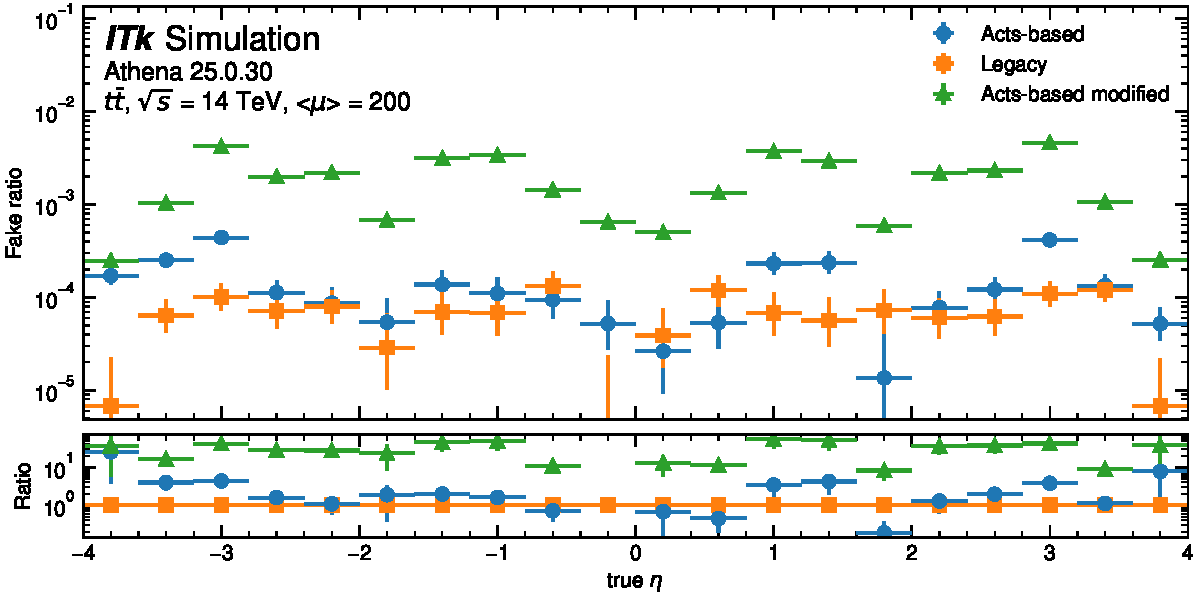
\includegraphics[width=1.0\linewidth]{parts/3_performance/12_itk-performance/figures/default_mod_ttbar_pu200_fake_vs_eta.pdf}
    \end{subfigure}
    \caption{Technical track efficiency (top) and fake ratio (bottom) as a function of true $\eta$ for \ttbar events with $\langle \mu \rangle = 200$ for the Acts-based and legacy chain.}
    \label{fig:perf/itk/eff-fake-ttbar}
\end{figure}

Figure \ref{fig:perf/itk/eff-fake-ttbar} shows the technical track efficiency and fake ratio as a function of true $\eta$ for \ttbar events with $\langle \mu \rangle = 200$ for the Acts-based and legacy chain.

Similar to what was observed for the single muon sample in Figure \ref{fig:perf/itk/eff-single-mu}, the Acts-based chain shows good efficiency for the endcap region $|\eta| > 1.5$, but significant inefficiency in the barrel region $|\eta| < 1.5$ compared to the legacy chain. The modified Acts-based chain shows a significant improvement in efficiency compared to the unmodified Acts-based chain in the barrel region and is consistently better than the legacy chain.

The fake ratio is comparable between the Acts-based and legacy chain. The modified Acts-based chain shows a significant increase in fakes on the order of a factor 10. This is due to the relaxed $\chi^2$ threshold for assigning measurements during track finding as it allows for more random measurement combinations to form fake tracks. Given this incease in fakes, the modified Acts-based chain cannot be the final solution for recovering the efficiency in the barrel region. The Acts-ITk team is currently working on identifying the cause of the inefficiency and how to improve it.

\section{Summary, conclusion and outlook}

The goal of the Acts-based chain is to be feature equivalent to the legacy chain and to achieve similar or better performance in terms of computation and physics. The work and results presented in this chapter are concerned with the main pass of track finding which reconstructs tracks from the primary interactions.

The track finding CPU performance of the Acts-based track reconstruction chain for the new inner tracking detector (ITk) of the ATLAS Phase-2 upgrade has been significantly improved during the work on this thesis. At the end of this first round of optimizations, the Acts-based track finding was about 8\% slower than the legacy chain, which is a significant improvement compared to the starting point. At the same time the physics performance is in agreement with the legacy  chain, when the $\chi^2$ threshold is relaxed for measurement selection during track finding.

The Acts-based chain is still missing a tuned track finding procedure for electrons and a more sophisticated ambiguity resolution algorithm to resolve cluster ambiguities and refit tracks based on this information. Apart from that, the chain shows inefficiencies for low momentum particles in the barrel region. This problem seems similar to the one observed with the OpenDataDetector (ODD) in Chapter \ref{ch:perf/odd}. A possible explaination for this is that material interactions are not properly modeled during reconstruction. In both cases the material is mapped to surfaces between the tracking layers and might not be placed in an optimal way leading to underestimated predicted position uncertainties on the sensors. This is an ongoing effort and the Acts-ITk team is currently working on improving the efficiency.

% current performance

% legacy
% track finding 3995949.24
% ambiguity solver 2737470.90
% total 6733420.14 (+68%)

% acts
% track finding 2310140.57
% pixel seeding 1931314.78
% strip seeding 478802.82
% ambiguity solver 233961.99
% total finding 4720258.17 (+18%)
% total 4954220.16 (+24%)

% acts modified
% track finding 2492342.54
% pixel seeding 1936541.73
% strip seeding 480295.06
% ambiguity solver 262040.74
% total finding 4909179.33 (+23%)
% total 5171220.07 (+29%)

\begin{table}[H]
    \centering
    \begin{tabular}{lcc}
        \hline
        \textbf{Chain} & \textbf{Rel. time w/o ambi} & \textbf{Rel. time w/ ambi} \\
        \hline
        Legacy & 1.00 & 1.68 (1.00) \\
        Acts-based & 1.18 & 1.24 (0.74) \\
        Acts-based modified & 1.23 & 1.29 (0.77) \\
        \hline
    \end{tabular}
    \caption{CPU performance of the track finding algorithm for the legacy and Acts-based chain as of April 2025 with Athena 25.0.30 (Acts v40.0.1) with and without ambiguity resolution.}
    \label{tab:perf/itk/track-finding-performance}
\end{table}

Table \ref{tab:perf/itk/track-finding-performance} shows the current CPU performance of the track finding algorithm for the legacy and Acts-based chain as of April 2025 with Athena 25.0.30 (Acts v40.0.1) with and without ambiguity resolution. This is the same version as used for the performance evaluation in Section \ref{sec:perf/itk/physics-performance}. The initial optimizations described in Section \ref{sec:perf/itk/cpu-performance} put the Acts-based chain within 8\% of the legacy chain. Recent developments have increased the gap again to 18\%. Applying the modified $\chi^2$ threshold for measurement selection during track finding increases the gap further to 23\%. Including the ambiguity resolution step, the Acts-based chain is 26\% faster than the legacy chain.

The Acts-ITk team will follow-up on new optimizations to the Acts-based track finding, trying to close the gap to the legacy chain. One focus will be on the triplet seeding algorithm, which appears to be the main CPU bottleneck due to the high fake rate. At the same time, the Acts implementation of the triplet seeding algorithm appears to be slower than the legacy one. Apart from that, the Acts-ITk team is working on integrating a new seeding algorithm which is expected to be faster and produce less fakes.
